\section{SCRUM}
\label{sec:SCRUM}

\rindex{\textbf{S}!SCRUM}The term itself comes from Rugby game, and describes a way of starting play again, in which players from each team come together and try to get control of the ball by pushing against each other and using their feet, when the ball is thrown in between their feet. 

\begin{figure}[!h]
\centering
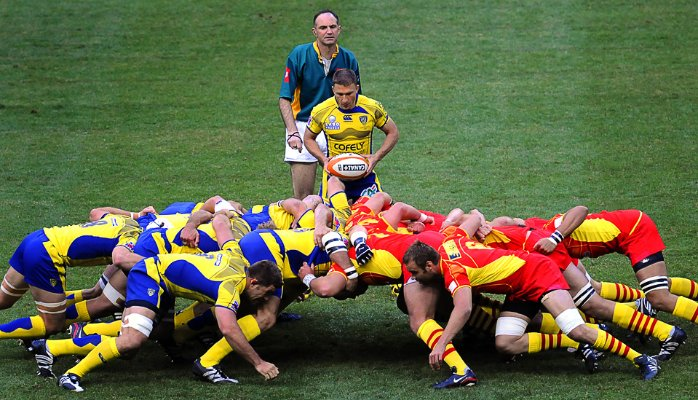
\includegraphics[width=0.8\linewidth]{realScrum}
\caption{\ttfamily{This is the real Scrum}}
\label{fig:realScrum}
\end{figure}

You can say '\textit{Jump everybody and let's kill them all!}' and millions will respond~\textemdash~yes! Well, this is \rindex{\textbf{W}!War}Rugby.

But you will suppose the SCRUM as a development approach, huh?!

\begin{figure}[!h]
\centering
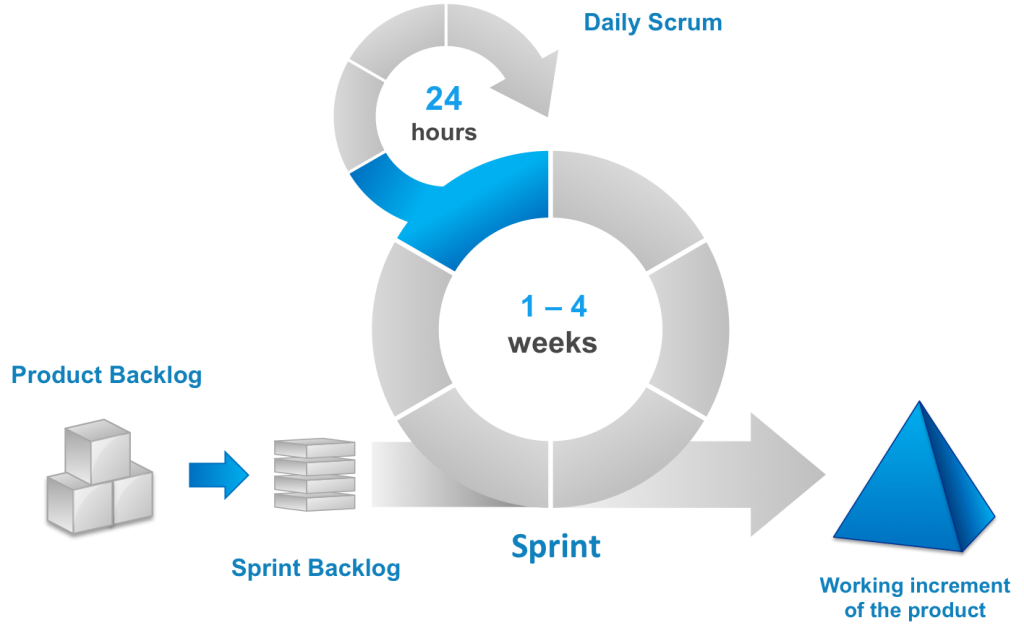
\includegraphics[width=1\linewidth]{scrumFramework}
\caption{\ttfamily{SCRUM Framework}}
\label{fig:scrumFramework}
\end{figure}

You will even say 'A software development methodology!', do you?!

This is not a methodology. 

This is a software development framework (a \rindex{\textbf{S}!Strategy}strategy) for managing product development, driven by agile principles. For being applied, the dev team already should have a development methodology.

Again, framework OVER a methodology.

\begin{verbatim}
ELSE
       Fail();
\end{verbatim}

See \rindex{\textbf{A}!Agile Software Development} Agile Software Development explanation [p.\pageref{sec:Agile Software Development}] \& agile principles at (\url{http://agilemanifesto.org/}) or GTFO.
